\begin{center}
\textsc{\Large Laboratorio 8}~\\
{\large Vídeo Juegos, Programación, Diseño}~\\
\emph{Menús e Interfaz de Juego}
\end{center}

\section{Pre-Laboratorio}
\todo[inline]{Por hacer.}

\section{Introducción}
\setlength\intextsep{0pt}
\begin{wrapfigure}[9]{l}{0.4\linewidth}
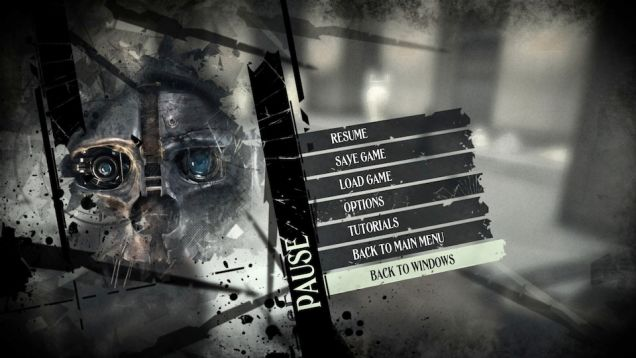
\includegraphics[width=\linewidth]{semana8/dishonored_menu.jpg} 
\caption{Menu de Inicio del video juego \emph{Disnohored}}
\end{wrapfigure}
Los vídeo juegos durante su ejecución presentan variados sistemas de interfaces, menús y pantallas de información al usuario, en la mayoría de los casos los juegos presentan como mínimo una pantalla de inicio con la opción de empezar el juego y salir de el mismo, otro menús muy común es el menú de opciones en el cual se presentan una variedad de personificaciones sobre ciertos parámetros del juego \cite{gb_optionsmenu}. Es usual que en plataformas como el computador personal se presenten mayor numero de opciones en el menú de opciones tales como opciones gráficas y de performance debido a la variada cantidad de configuraciones de hardware, en otras plataformas como las consolas es común que solo se presenten modificaciones sobre el audio del juego, dificultad o re-configuración de los controles de juego.

\section{Menus e Interfaces Comunes}
Las necesidades de interfaces, pantallas y menús cambian según los requerimientos de diseño de cada juego, sin embargo se presentan acá los componentes de interfaz y menús encontradas en la mayoría de los vídeo juegos actuales.
\subsection{Menu de Inicio}
\subsection{Menu de Opciones}
\subsection{Menu de Partidas (\emph{Save Games})}
\subsection{HUD (\emph{Heads-Up Display})}
\subsection{Creditos}

\section{Actividad}
\todo[inline]{Por hacer.}